\chapter{Non-linear elasticity equation --3D -- Loaded elastic curve}

\modinfo{Files}{u\_turn.grd}
\modinfo{Solvers}{\Idx{ElasticSolve}}
\modinfo{Tools}{\Idx{ElmerGUI}}
\modinfo{Dimensions}{3D, Transient}
\modinfo{Author}{Peter R{\aa}back}


\subsection*{Case definition}

An elastic U-shaped cylinder is pressed from its ends such that
the object faces large displacements. The material properties of
stainless steel are used. Problem is to gradually increase the displacement
and visualize the increase of stresses. The problem requires the use
of solver capable of dealing with large displacement.


\subsection*{Solution procedure}

The mesh is given in ElmerGrid format in file \texttt{u\_turn.grd},
load this file.
\ttbegin
File 
  Open -> u\_turn.grd
\ttend
You should obtain your mesh and may check that it consists of 12288 trilinear elements and 13585 nodes.
\begin{figure}[h!]
\begin{center}
  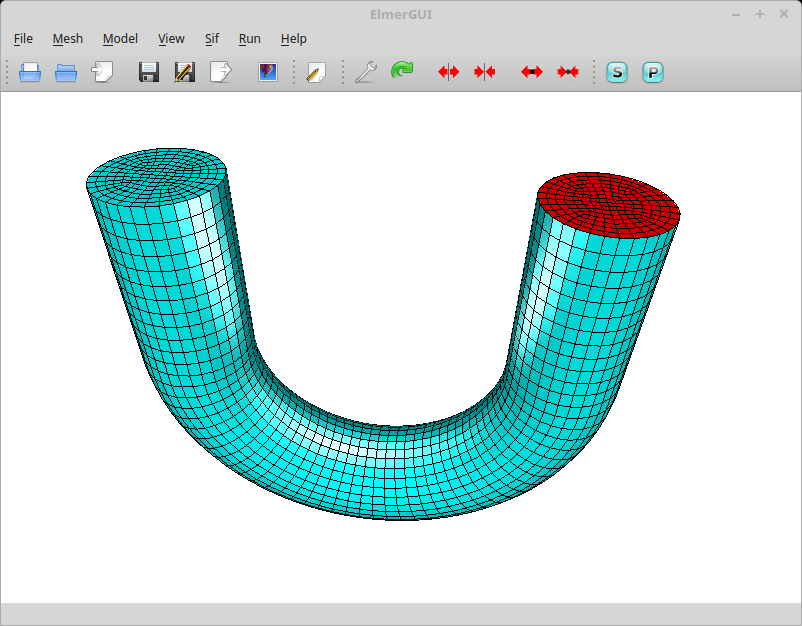
\includegraphics[width=0.6\textwidth]{UturnElmerGUI}
  \caption{The mesh used in the computations as shown in ElmerGUI.}
  \label{fig:UturnElmerGUI}
\end{center}
\end{figure}

After we have the mesh we start to go through the Model menu from the top to bottom. 
In the Setup we choose things related to the whole simulation such as file names, 
time stepping, constants etc.
The simulation is carried as a transient problem in 3-dimensional Cartesian
coordinates. The inertial forces of no importance so we could as well scan through a set of steady state
loading conditions. We choose the time step such that the total time being simulated is 1~s.
We assume that the original mesh (with diameter 0.6 is given units of cm. Hence we need to scale the
system down to work in SI units. 
\ttbegin
Model
  Setup 
    Simulation Type = Transient
    Timestep Sizes = 0.05
    Timestep Intervals = 20
    Coordinate Scaling = 0.01
\ttend

In the Equation section we choose the relevant equations which in this case only includes 
the \texttt{Nonlinear elasticity} equation.
We have just one body and therefore its easy to assign 
the Equation and Material to it directly.
We can use linear system solvers we are happy to use the defaults. One may however, try out different
preconditioners (ILU1,\ldots) or more efficient iterative methods (BiCGStabl), for example.
\ttbegin
Model
  Equation
    Name = Elasticity
    Apply to Bodies = 1
    Nonlinear elasticity
      Active = on
      Edit Solver Settings
        Calculate Stresses = on
        Calculate Principal = on
    Add 
    OK
\ttend        
Here we choose the stainless steel from the material library.
You may click trough the material parameters of the various solvers to ensure that
the properties are indeed as they should be. Any consistent set of units may be used in Elmer.
The natural choice is of course to perform the computations in SI units. 
\ttbegin
Model
  Material
    Material library    
      Austenitic stainless steel (AK Steel 201)
    Apply to Bodies = 1 
    Add
    OK
\ttend

There are no body forces and convergence should be easily obtained with the default 
initial condition i.e. zero for all fields. Hence we don't need to toggle these subitems. 

We need to type now boundary conditions that we will later assign with the mouse to some surfaces.
We set boundary conditions for both ends of the hook such that
they close with respect to each other with time. The distance travelled in 1~s will be set to
0.006~m i.e. to same as the radius. The other displacement components are set to zero.  
To type in the multiline expressions for the boundary condition just press \texttt{Enter}
\texttt{Displacement 1} checkbox.
Note that the semicolon is an alternative separator
to line break. 
\ttbegin
Model
  BoundaryCondition
    Name = MovingRight
    Nonlinear elasticity
      Displacement 1 = Variable "time"
        Real MATC "0.006*tx"
      Displacement 2 = 0.0
      Displacement 3 = 0.0
    Add
    New

    Name = MovingLeft 
    Nonlinear elasticity
      Displacement 1 = Variable "time"
        Real MATC "-0.006*tx"
      Displacement 2 = 0.0
      Displacement 3 = 0.0
    Add 
\ttend   

The conditions may also be assigned to boundaries in the Boundary condition menu, or 
by clicking with the mouse. Here we use the latter approach as that spares us of the 
need to know the indexes of each boundary.
\ttbegin
Model
  Set boundary properties
    Choose negative x end -> set boundary condition "MovingRight"
    Choose positive x end  -> set boundary condition "MovingLeft"
\ttend

For the execution 
ElmerSolver needs the mesh files and the command file. We have now basically defined
all the information for ElmerGUI to write the command file. After writing it we may also visually 
inspect the command file.
\ttbegin
Sif 
  Generate
  Edit -> look how your command file came out  
\ttend

Before we can execute the solver we should save the files in a directory. The project includes
all the files needed to restart the case.
\ttbegin
File 
  Save Project
\ttend

After we have successfully saved the files we may start the solver
\ttbegin
Run
  Start solver
\ttend
A convergence view automatically pops up showing relative changes of each iteration.
As there are 20 time steps the convergence will be shown for each time step.
You can start looking at the results already after a few time steps. The whole simulation
takes a few minutes. 
\ttbegin
Run
  Start ParaView
\ttend


\begin{figure}[h!]
\begin{center}
  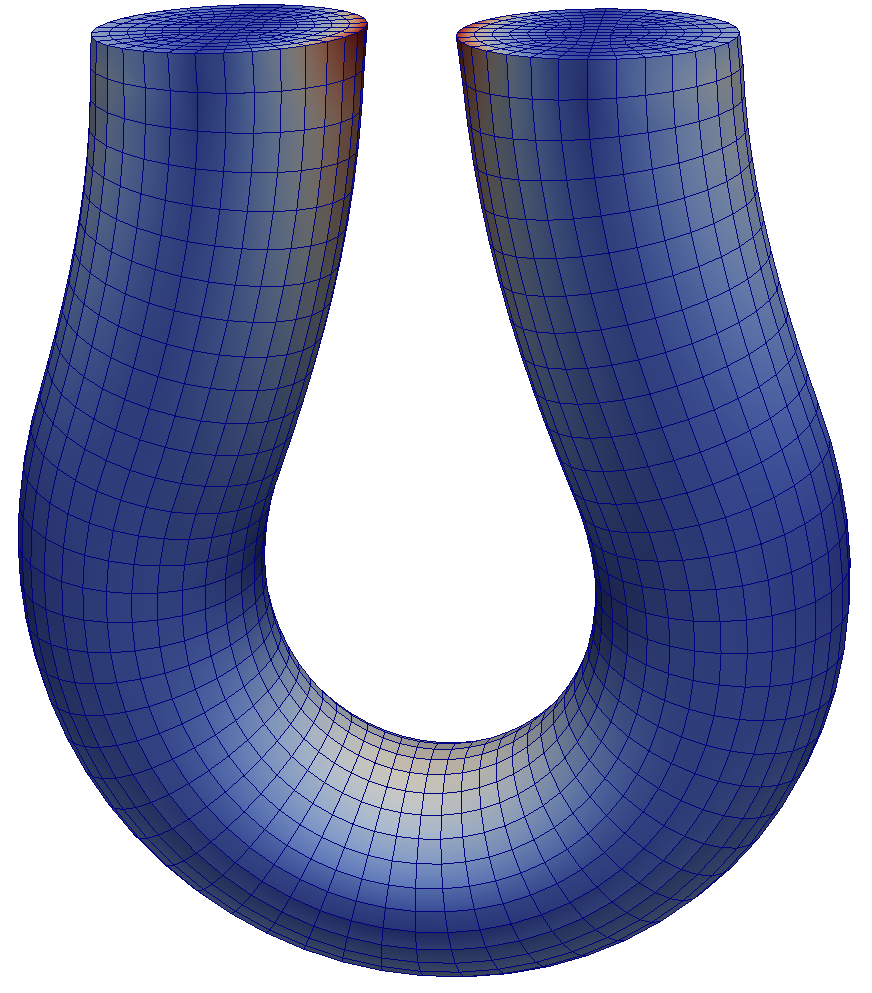
\includegraphics[width=0.5\textwidth]{UturnVonMisesStressMesh}
  \caption{The final state of the deformed curve. Color shows the resulting von Mises stresses.}
  \label{fig:UturnVonMisesStress}
\end{center}
\end{figure}

In reality the material could break at some point. Here we have assumed a linear material law
even though the geometric displacement makes the equation non-linear. 


\subsection*{Alternative task: Rotating square profile}

You may perform the tutorial with an alternative geometry: \texttt{square\_profile.grd}.
Follow almost the same logic except now we rotate the ends of the beam.

We need to enforce rigid body rotations to the ends of the mesh. The following
types of Dirichlet conditions need to be implemented
\begin{equation}
  \begin{array}{ll}
    u_x = & ( \cos(\phi) - 1)x - \sin(\phi)y ) \\
    u_y = & ( \cos(\phi) - 1)y + \sin(\phi)x )     
  \end{array}
\end{equation}
These can be set using the following \texttt{MATC} function
\ttbegin
  Displacement 1 = Variable "time, Coordinate"
    Real MATC "(cos(tx(0)*pi)-1.0)*tx(1)-sin(tx(0)*pi)*tx(2)
  Displacement 2 = Variable "time, Coordinate"
    Real MATC "(cos(tx(0)*pi)-1.0)*tx(2)+sin(tx(0)*pi)*tx(1)
\ttend 
Note that the argument to \texttt{MATC} is always called \texttt{tx} and it holds the
parameters in the given order. In this case component "0" refers to \texttt{time}, component "1" to
\texttt{Coordinate 1} (i.e. x), and component "2" to \texttt{Coordinate 2} (i.e. y). 
The multiplier for the trigonometric functions is $\pi$ which means that a revolation of
180 degrees is performed in 1 second. 
 
\begin{figure}[h!]
\begin{center}
  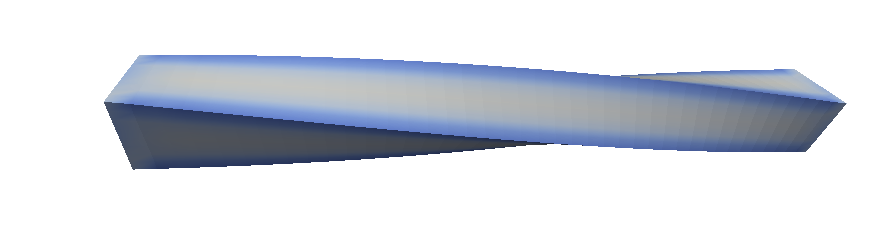
\includegraphics[width=0.6\textwidth]{RotatingProfile50}
  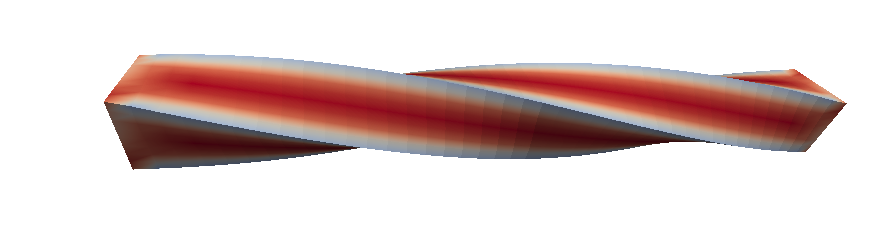
\includegraphics[width=0.6\textwidth]{RotatingProfile100}
  \caption{A square profile being rotated from one end by 90 and 180 degrees. Color shows the von Mises stresses.}
  \label{fig:RotatingProfile}
\end{center}
\end{figure}



\vfill
\mbox{}
